\documentclass{beamer}

%\usepackage[utf8]{inputenc}
\usepackage[T1]{fontenc}
\usepackage{fontspec}
\usepackage[brazil]{babel}
\usepackage{listings}
\usepackage{graphicx}
\usepackage{color}
\definecolor{editorGray}{rgb}{0.95, 0.95, 0.95}
\definecolor{editorOcher}{rgb}{1, 0.5, 0} % #FF7F00 -> rgb(239, 169, 0)
\definecolor{editorGreen}{rgb}{0, 0.5, 0} % #007C00 -> rgb(0, 124, 0)
\usetheme[outer/progressbar=foot]{Metropolis}
\setsansfont[BoldFont={Source Sans Pro Semibold},Numbers={OldStyle}]{Source Sans Pro}

%\makeatletter
%\def\verbatim@font{\ttfamily}
%\makeatother

\lstset{%
    % Basic design
    backgroundcolor=\color{editorGray},
    basicstyle={\scriptsize\ttfamily},   
	%basicstyle={\scriptsize},   
    frame=l,
    % Line numbers
    xleftmargin={0.75cm},
   % numbers=left,
    stepnumber=1,
    firstnumber=1,
    numberfirstline=true,
    % Code design   
    keywordstyle=\color{blue}\bfseries,
    commentstyle=\color{darkgray}\ttfamily,
    ndkeywordstyle=\color{editorGreen}\bfseries,
    stringstyle=\color{editorOcher},
    % Code
    language=csh,
    alsodigit={.:;},
    tabsize=2,
    showtabs=false,
    showspaces=false,
    showstringspaces=false,
    extendedchars=true,
    breaklines=true,
    morekeywords={
    	abstract, event, new, struct,
    	as, explicit, null, switch,
    	base, extern, object, this,
    	bool, false, operator, throw,
    	break, finally, out, true,
    	byte, fixed, override, try,
    	case, float, params, typeof,
    	catch, for, private, uint,
    	char, foreach, protected, ulong,
    	checked, goto, public, unchecked,
    	class, if, readonly, unsafe,
    	const, implicit, ref, ushort,
    	continue, in, return, using,
    	decimal, int, sbyte, virtual,
    	default, interface, sealed, volatile,
    	delegate, internal, short, void,
    	do, sizeof, while,
    	double, lock, stackalloc,
    	else, long, static,
    	enum, namespace, string
    },
    literate={ç}{{\c{c}}}1 {é}{{\'e}}1 {á}{{\'a}}1 {ã}{{\~a}}1 {ó}{{\'o}}1 {í}{{\'i}}1
}

\begin{document}
\title{Programação Básica em C\# para Unity - Implementação do jogo Breakout}   
\author{Bruno dos Santos de Araújo, MSc} 
\date{\today} 

\frame{\titlepage} 

\frame{\frametitle{Sumário}\tableofcontents} 
\section{Introdução}

\begin{frame}[fragile]{Introdução}

\begin{itemize}
	\item O jogo Breakout foi lançado em 1976 pela Atari para arcades, em 1972, e em 1986 foi lançado Arkanoid, pela Taito, que expandiu o conceito original adicionando power-ups, diferentes tipos de tijolos e visuais diferentes.
	\item O objetivo do jogo é quebrar todos os tijolos sem deixar a bolinha cair na parte de baixo da tela.

\end{itemize}

\begin{columns}
	\begin{column}{0.5\textwidth}
		\begin{figure}
			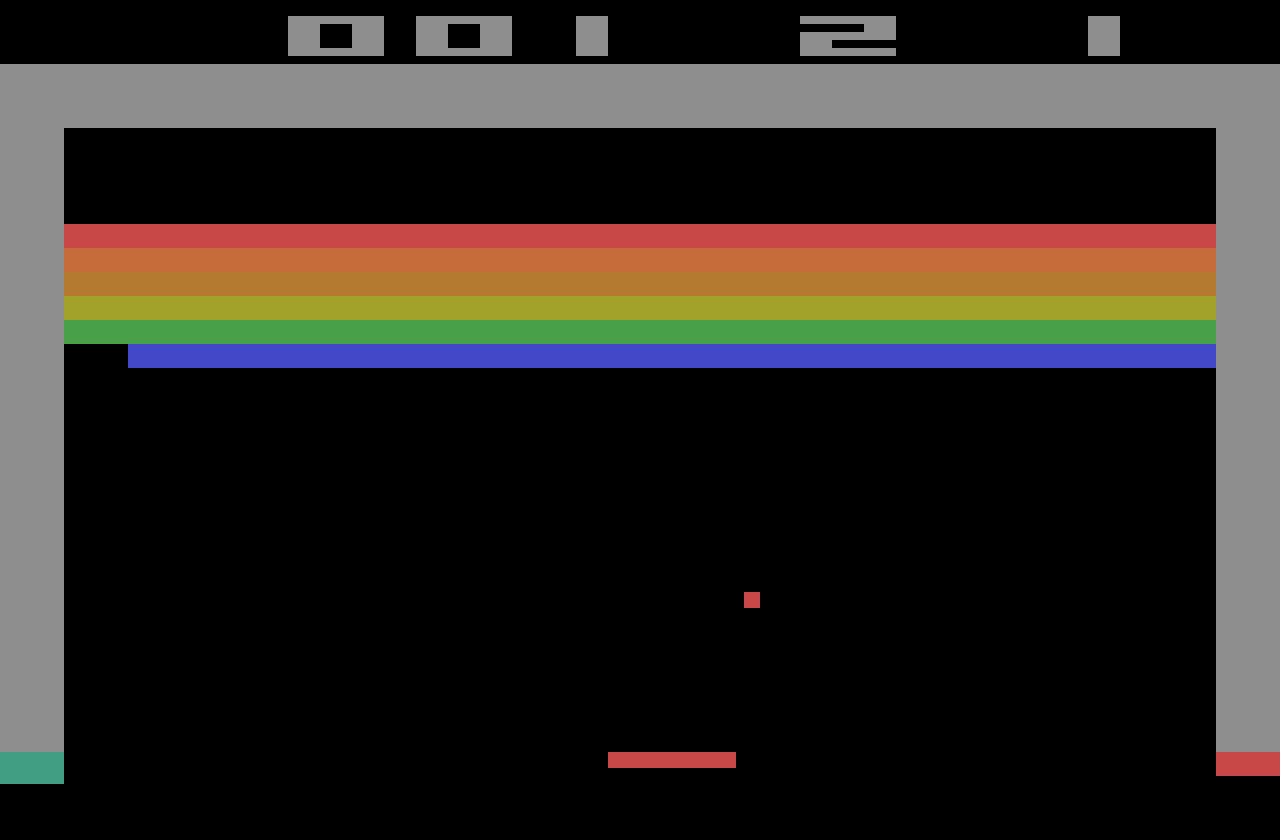
\includegraphics[width=0.75\textwidth]{breakout.png}
			\caption{Breakout (Atari 2600)}
		\end{figure}
	\end{column}
	\begin{column}{0.5\textwidth}
		\begin{figure}
			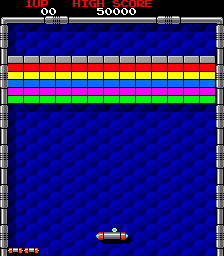
\includegraphics[width=0.55\textwidth]{arkanoid.png}
			\caption{Arkanoid (Arcade)}
		\end{figure}	
	\end{column}	
\end{columns}
\end{frame}

\section{Implementação do player}
\section{Implementação da bolinha}
\section{Implementação dos tijolos}


%\begin{frame}[fragile]{Estrutura de um MonoBehaviour}
%	\begin{itemize}
%		\item \verb|OnDestroy()|: chamada quando o objeto é destruído, seja quando a cena é descarregada ou usando \verb|Destroy()| diretamente.
%		\begin{itemize}
%			\item Menos comumente utilizada, mas útil pra quaisquer tarefas de limpeza quando o objeto é destruído.
%		\end{itemize}
%	\end{itemize}
%	\begin{lstlisting}
%private void Destroy()
%{
%	RemoveFromEnemyList();
%}
%	\end{lstlisting}
%\end{frame}
%
%\begin{frame}[fragile]{Exemplo da ordem de execução dos scripts}
%	
%\begin{columns}
%\column{0.5\textwidth}
%\begin{lstlisting}
%private void Awake() {
%	Debug.Log("Awake()");
%}
%
%private void Start() {
%	Debug.Log("Start()");
%}
%
%private void OnEnable() {
%	Debug.Log("OnEnable()");
%}
%\end{lstlisting}
%
%\column{0.5\textwidth}
%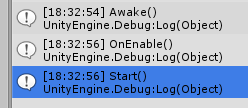
\includegraphics{executionorder.png}
%\end{columns}
%	
%\end{frame}


\end{document}

